\section{Observational site}

The field campaign occurred in the west face of the Grand Colon mountain (2394~meters) in the Belledonne Massif, 15~km East of Grenoble. A topographic map of the area is shown in figure~\ref{fig:obs_site}, where the measuring site is marked with a green star. %The west face of the mountain was selected because it gives direct exposure to solar radiation during the afternoon. This is ideal for katabatic winds to form because the ground cools down after the sun goes down.

\begin{figure}[!ht]
  \begin{center}
  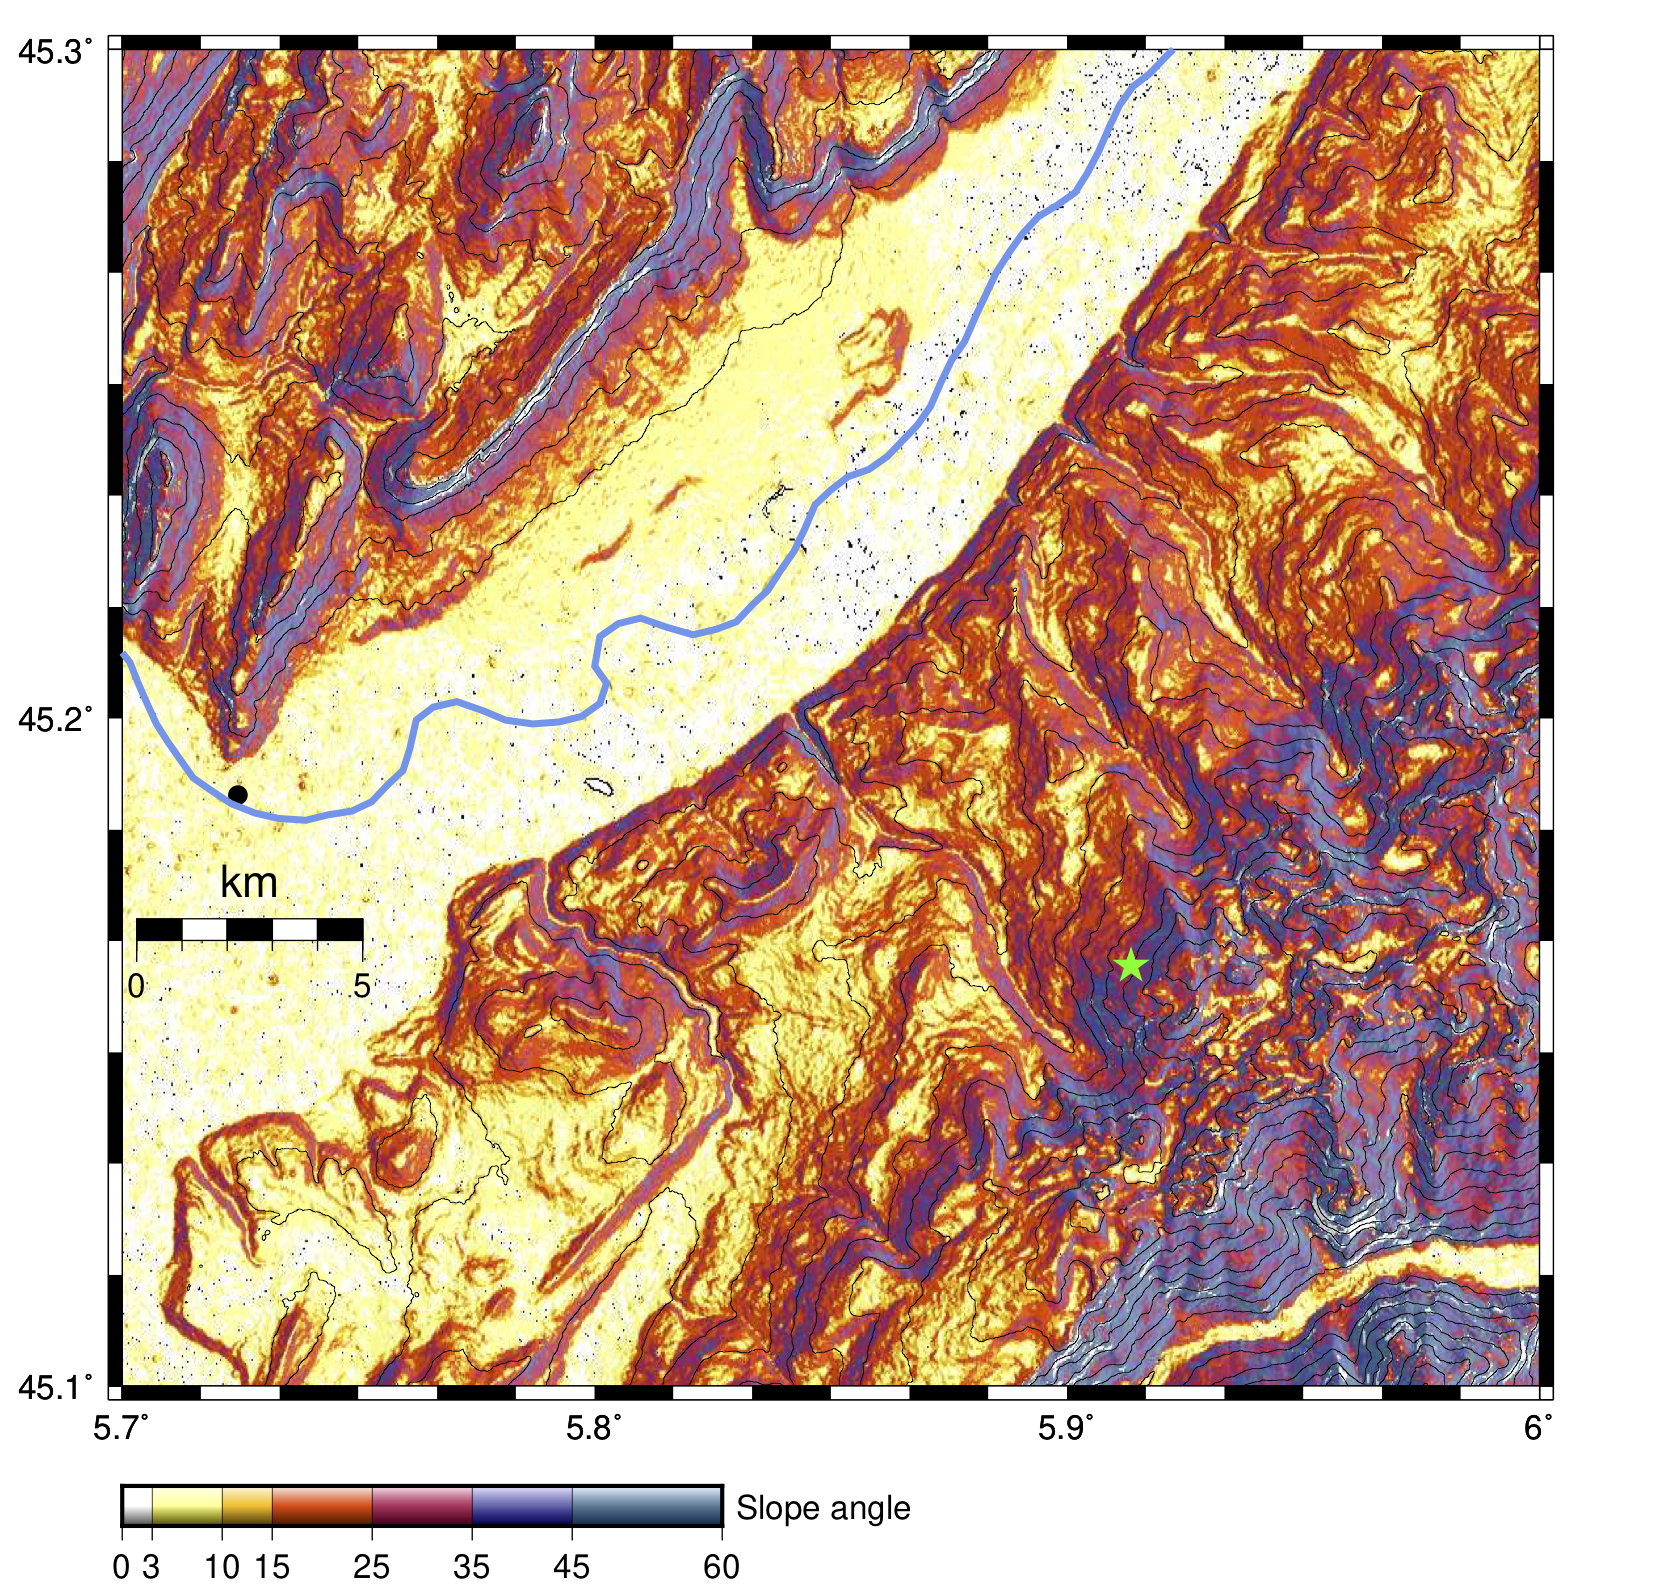
\includegraphics[width=0.8\textwidth]{fig/chapter_3/grenoble_slopes_C100.png}
  \caption{Topographic map showing the slopes of the region. The green star marks the position of the measuring site. The black dot marks the localisation of Grenoble. Data obtained from Shuttle Radar Topography Mission using the GMTSAR processing system~\citep{sandwell2011gmtsar}.}
  \label{fig:obs_site}
  \end{center}
\end{figure}

The meteorological station was located at 1770~m height, located in an alpine pasture area (low vegetation and sparse rocks or pebbles) above the forest area and
has a relatively homogeneous slope, which fulfils the essential characteristics for a detailed analysis of the physical process~\citep{blein2016observation}. In particular, the ground was covered by a layer of snow which thickness decreased during the field campaign. The average slope of the site is around 30~$\degree$.

\section{Instrumentation} \label{instrumentation}

The instruments placed in the field were mounted into two masts. The principal mast measured 10~m and on it were mounted 11 sonic anemometers and 10 thermocouples (see figure~\ref{fig:mast}). There was a smaller mast (2~m) with a meteorological station placed a few meters apart from the main mast. 

On the small mast, or meteorological mast, there were the following instruments installed: 
\begin{itemize}
    \item CS100 standard barometer (Campbell Scientific), for atmospheric pressure.
    \item CNR1 net radiometer sensor (Campbell Scientific), for short and long wavelength radiation fluxes.
    \item IR120 infrared radiometer (Campbell Scientific), for measuring the longwave radiation flux emitted by the ground.
    \item CS125 temperature and relative humidity sensor (Campbell Scientific).
    \item SR50 sonic ranging sensor (Campbell Scientific), for measuring the position of the sensors relative to the ground.
\end{itemize}

In the big mast there were four types of anemometers with different characteristics and only one type of thermocouple. The anemometers were the CSAT3 and CSAT3B~\footnote{The CSAT3B is the most recent version of the CSAT3.} 3-D sonic anemometers manufactured by Campbells Scientific, which measure three components of the wind with a frequency of 20~Hz. In total there were five CSAT3 and only one CSAT3B. Also, we used four Windsonic 2-D sonic anemometers manufactured by Gill Instruments. This anemometer measures two components of the mean wind that are aligned to the "plane" of the instrument. At the top of the mast, a Windmater Pro Sonic Anemometer (from Gill Instruments) was placed. As the CSAT3, it measured three components of the wind with a frequency of 20~Hz. The Table~\ref{tab:intruments_anemometers} shows the initial heights of the the anemometers.

\begin{table}[!ht]
    \centering
    \begin{tabular}{ | l | c | c | c |}
    \hline
    \textbf{Instrument} & \textbf{Variables measured} &  \textbf{Frequency (Hz)} & \textbf{Initial height (m)} \\ [0.5ex]  \hline\hline
    CSAT3B & \multirow{6}{*}{(u,v,w) and Temp.} & \multirow{6}{*}{20} & 0.035 \\
    CSAT3 No.5 &  &  & 0.36 \\
    CSAT3 No.4 &  &  & 0.67 \\
    CSAT3 No.3 &  &  & 1.16 \\
    CSAT3 No.2 &  &  & 1.57 \\
    CSAT3 No.1 &  &  & 1.98 \\
    \hline
    Windsonic 2D No.3 & \multirow{4}{*}{(u,v)} & \multirow{4}{*}{0.003} &  2.7\\
    Windsonic 2D No.2 &  &  &  3,69\\
    Windsonic 2D No.1 &  &  &  5.42\\
    Windsonic 2D No.0 &  &  &  7.02\\
    \hline
    Windmaster Pro & (u,v,w) and Temp. & 20 & 8.97 \\
    \hline
    
    \end{tabular}
    \caption{Specification for the different anemometers installed.}
    \label{tab:intruments_anemometers}
\end{table}

An important aspect of the anemometers is their orientation and alignment with respect to the slope. In this case, we aligned all the anemometers in a manner that the horizontal wind components of the instruments were parallel to the slope surface and the vertical wind component perpendicular to the surface (figure~\ref{fig:mast_pics} shows how the instruments are tilted, following the slope of the mountain). The orientation of the instruments was different for the CSAT3, the Windsonic 2-D and the Windmaster Pro. The CSAT3 and CSAT3B were oriented towards the south (180~$\degree$ North off-set), in a way that the $v$ component of the wind was facing the slope (eastwards) and the $u$ was facing the right side of the slope (southwards). The Windsonic 2-D was oriented towards the West (270~$\degree$ North off-set) in a manner that the negative $u$ component was facing the slope (facing the towards the valley, i.e. towards the West). And the Windmaster Pro was facing towards the slope or facing East (90~$\degree$ North off-set).

\begin{figure}[!ht]
  \begin{center}
  \includegraphics[width=0.6\textwidth]{fig/chapter_3/Montage.jpg}
  \caption{Scheme of the principal mast with the position and label of the instruments.}
  \label{fig:mast}
  \end{center}
\end{figure}

\begin{figure}[!ht]
    \centering
    \begin{subfigure}[b]{0.308\textwidth}
        \includegraphics[width=\textwidth]{fig/chapter_3/foto_1_small.jpg}
    \end{subfigure}
    \quad
    \begin{subfigure}[b]{0.4\textwidth}
        \includegraphics[width=\textwidth]{fig/chapter_3/foto_3_small.jpg}
    \end{subfigure}
    \caption{To the left, we can see a picture of the principal mast viewed from the side and at the back is possible to see the small mast. In the picture in the right we can see a zoom on the CSAT3 anemometers viewed from bellow.}
    \label{fig:mast_pics}
\end{figure}

Spread along the mast, there are ten thin thermocouples, that were used to measure the air temperature with a minimal intrusion at high frequency (20~Hz). The initial heights of these instruments are shown in table~\ref{tab:intruments_thermocouples} and can be seen in figure~\ref{fig:mast} at the left of the mast, opposite to the anemometers.

\begin{table}[!ht]
    \centering
    \begin{tabular}{ | l | c | c | c |}
    \hline
    \textbf{Instrument} & \textbf{Variables measured} & \textbf{Frequency (Hz)} & \textbf{Initial height (m)} \\ [0.5ex]  \hline\hline
    Thermocouple No.1 & \multirow{10}{*}{Temperature} & \multirow{10}{*}{20} &  0.05\\
    Thermocouple No.2 & &  &  0.13\\
    Thermocouple No.3 & &  &  0.21\\
    Thermocouple No.4 &  &  &  0.29\\
    Thermocouple No.5 & &  &  0.38\\
    Thermocouple No.6 &  &  &  0.47\\
    Thermocouple No.7 & &  &  2.53\\
    Thermocouple No.8 &  &  &  3.52\\
    Thermocouple No.9 &  &  &  5.26\\
    Thermocouple No.10 &  &  & 6.84 \\
    \hline
    
    \end{tabular}
    \caption{Specifications of the Thermocouples.}
    \label{tab:intruments_thermocouples}
\end{table}

%In the middle, there is a radiometer used to measure the radiant flux. Finally, there is an ultrasonic instrument installed in the station to record the height of the snow cover (snow-covered ground was expected in the measuring site). This is important because the snow decreases the height between the ground and the instruments, which is an important parameter in the calculations.

\section{Field campaign}

The field campaign could only take place during certain weather conditions and during winter. For this reason, we couldn't establish a certain date for it. First of all, winter is the season when the occurrence of katabatic winds event is greater because of the cold temperatures in the mountains. Also, the other important factor, as mentioned in section~\ref{sec:katabatic_winds}, is that the presence of mesoscale wind systems can overshadow or inhibit the formation of katabatic winds. For this reason, an ideal weather condition for measuring katabatic winds is during anticyclonic events, in which mesoscale wind systems are weak, the ski is clear and the air is cold.

During the month of February, between the 10th and the 28th,  Grenoble had anticyclonic weather conditions that were brought by three high-pressure systems that passed over the region during this period of time, these were named: Dorit, Erika and Frauke~\citep{highslist}. This meteorological window allowed us to carry out the field campaign. In total, the instruments took measurements for 17 days.

\section{Data processing}

In total around 11.5~GB were obtained during the campaign, only taking into account the anemometers, the thermocouples and the meteorological station. The processing of the data depended on the instrument and its frequency of operation. 

\subsubsection{CSAT3 and Windmaster Pro}

For the CSAT3 anemometers and the Windmaster Pro we used EddyPro, which is a software that uses the eddy covariance method to compute atmospheric fluxes of certain trace gases, heat flux and energy~\citep{burba2013eddy}. EddyPro computes the averages of each of the components of the wind and the temperature for a certain period of time which we choose. After this, it computes the fluctuations (turbulent parts) of the variables and computes the covariance between them. There are multiple choices for software that can do this but EddyPro integrates different functions and methods that improve the quality of the output. 

The raw data of the sonic anemometers is in ASCII format, which EddyPro can read only pointing out what are the columns corresponding to each variable and each instrument. For this also we have to specify the height of the instruments with respect to the ground, the orientation of the instruments with respect to the north, the type of average to compute and the period for computing the average. 

Due to the number of days the instruments were operating and the high frequency of acquisition, it was convenient to use a relatively large period for averaging to try to identify the days when there were good conditions for katabatic winds to form. For this reason, we processed the data doing 30 minutes averages for both the CSAT3 anemometers and the Windmaster Pro. This type of average works as a low-pass filter for the raw high-frequency signal, where all the turbulent fluctuations of the variables are lost. For this reason, is only convenient to use this 30~minutes averaged data to identify potential good periods with the required conditions and not to analyse the turbulent characteristics of the flow

After identifying three potentially good nights for katabatic winds episodes, we went back to EddyPro and processed the data using a 5~minutes average period, which works better to analyse the turbulent characteristics of the flow and the respective fluxes. In particular we computed the sensible heat flux ($\overline{w'\theta'}$), the momentum flux ($\overline{u'w'}$) and the turbulent kinematic energy (TKE).

\subsubsection{Thermocouples and Windsonic 2-D anemometers}

As mentioned before, the raw data of the thermocouples have a frequency of 20~Hz, and the Windsonic anemometers record 5~minutes-averages. Both instruments are incompatible with EddyPro because they do not measure wind velocity and temperature simultaneously, which makes them unfit for the eddy covariance method used by the software. This is why for these instruments it was necessary to write a script to compute the average at a different frequency. As with the 3-D sonic anemometers, first, we did a 30 minutes average of the data for both type of instruments, to be able to analyse and detect the best nights to observe katabatic wind. After determining the ideal nights, we performed 5~minute averages of the raw data.

\section{Temperature comparison between thermocouples and CSAT3 anemometers}

With the 30~minute averaged data, we compared the temperature measured by the CSAT3 instruments with respect to the temperature of the thermocouples. We did this to verify that the temperature of the sonic anemometers was consistent because this temperature is used to compute the heat fluxed, which is an important aspect of the flow. 

For this, we selected a thermocouple and a CSAT3 placed at the same height or very close in height to one another. From figure~\ref{fig:mast} and the tables~\ref{tab:intruments_anemometers}~and~\ref{tab:intruments_thermocouples} is possible to see that the CSAT3B and the Thermocouple No.1 are very close in height, only 1.5~cm of difference. Also, the CSAT3 No.5 and the Thermocouple No.5 are very close with 2~cm of difference. To this data, we did a calibration plot of the temperature of both instruments (CSAT3 vs Thermocouple) and computed the correlation coefficient. This gave us an insight into how well the measurements of temperature obtained from the CSAT3 are. 

\section{Wind speed comparison between CSAT3 and Windsonic 2D anemometers}

As in the previous section, and because we have three types of anemometers installed in the mast, it was necessary to check that the measurements of the wind speed were consistent between instruments. For this, we selected the closest CSAT3 to the WINDSONIC 2D no.3, which is the closest to the ground from the Windsonic's installed. The CSAT· No.1 is the closest one to this instrument, with a vertical separation of 72~cm. For this we only compared mean the wind speed of both instruments, disregarding the wind direction, and did a scatter plot for both instruments, computing the correlation coefficient. 

The comparison between the Windmaster Pro and the Windsonic 2-D was not performed because the separation between the closest Windsonic anemometer to the wind master on the top is of around 2~m. 

\section{Wind direction correction}

When analysing the wind direction data from all the anemometers we saw that there where inconsistencies with the wind direction of the CSAT3B anemometer, placed at the bottom of the mast. We found out that there was a systematic deviation of $+90\degree$ with respect to the other CSAT3 instruments, and the variation of the angle was inverted with respect to the other CSAT3's. To identify this we did a calibration plot (see appendix~\ref{app:wind_dir}) between the wind direction of the CSAT3B and the CSAT3 No.5, which is the closest one to the CSAT3B, and proposed a correction, which we implemented when analysing the data.

\section{Ground temperature calculation}

Using the data from the radiometer CNR1 installed in the small mast, in specific the longwave emitted radiation from the ground (considered as a black body), we computed the ground temperature using the Stephan-Boltzmann Law:

\begin{equation}
    I = \sigma T^4, 
\end{equation}

\noindent which relates the radiant emittance with respect to the temperature of a body, where $\sigma = 5.67 \times 10^{-8} W m^{-2} K^{-4}$, is the Stephan-Boltzmann, and $T$ is the body temperature. Solving for $T$ and using the longwave emitted radiation from the ground as $I$, we computed the time series of the temperature of the ground.

%With the ground temperature, we computed the temperature gradient between the ground and the CSAT3 No.4. We choose the CSAT3 No.4 because is placed in the middle of the CSAT3 array and is not to close to the ground. To compute the gradient we did the operation:

%\begin{equation}
%    \text{grad}_z T = \frac{T_{csat} - T_{grd}}{h_{csat} - h_{grd}},
%\end{equation}

%\noindent where $T_{csat}$ and $T_{grd}$ are the CSAT3 No.4 and ground temperature respectively at certain time. The height of both instruments are the variables $h_{csat}$ and $h_{grd}$ respectively. Because this height is measured with respect to the ground, $h_{grd} = 0$, and we use the corresponding value of the height of the CSAT3 No.4 at each particular time. 

\section{Criterion for choosing the nights to analyse}

The criteria for detecting katabatic winds can be summarized in two important aspects: Temperature gradient and external forcing. The temperature gradient refers to the vertical temperature gradient between the ground and the air. When there is a strong vertical gradient, where the ground is colder than the air above it, the gradient forms a stable stratification of the air. During the night is when the ground is colder because of the absence of incident solar radiation, which decreases the ground temperature, and therefore, starts to cool down the air that is in contact with, creating the conditions for the katabatic wind to form. For this reason, we restricted our analysis to the nights of the field campaign. 

The other aspect is that there should not be signs of externals forcing or strong winds blowing, which can inhibit the formation of the katabatic wind. A way to detect this is when the data suddenly registers peaks in the wind speed for all the different heights. Also, these external forcing have the characteristic of carrying hotter air compared with the ambient temperature of the air. This means that when the data displays sudden jumps in wind speed and air temperature, is due to an external weather system that is passing through the region, and the possibility of detecting katabatic flows is low.

The first filter used to detect the optimal nights was direct observation done during the campaign, where it was registered the atmospheric conditions and the intensity of the wind in the measuring site. This gave us an insight into the potentially good nights with low wind speeds and allow us to focus the analysis in them.

Finally, when these conditions are gathered, we should be able to see a maximum in the mean wind speed profile close to the ground, with a downslope wind. This is the signature of katabatic winds.